\section{Explainable AI and dementia}

\newcommand{\neuron}[3]{
    \node[circle, draw=black, fill=#2] (#1) at #3 {};
}


\begin{frame}{Theoretical background}
    \begin{tikzpicture}
        \node[] at (-5.25, -3.5) {};
        \node[] at (5.25, 3.5) {};

        \node[
            draw=black,
            fill=cyan!15,
            minimum height=3cm,
            minimum width=4.3cm
        ] (model) at (0, 1) {};

        \def\hsep{0.7}
        \def\vsep{0.5}
        \def\edgecolor{gray}
        \def\edgeopacity{0.5}
        \def\neuroncolour{gray}

        \only<1>{
            \node[
                anchor=south,
                font=\small
            ] at (model.north) {Artificial neural network};

            \neuron{n00}{\neuroncolour}{($ (model) + (-2 * \hsep, -2 * \vsep) $)}
            \neuron{n01}{\neuroncolour}{($ (model) + (-2 * \hsep, -\vsep) $)}
            \neuron{n02}{\neuroncolour}{($ (model) + (-2 * \hsep, 0) $)}
            \neuron{n03}{\neuroncolour}{($ (model) + (-2 * \hsep, \vsep) $)}
            \neuron{n04}{\neuroncolour}{($ (model) + (-2 * \hsep, 2 * \vsep) $)}

            \neuron{n10}{\neuroncolour}{($ (model) + (-\hsep, -1.5 * \vsep) $)}
            \neuron{n11}{\neuroncolour}{($ (model) + (-\hsep, -0.5 * \vsep) $)}
            \neuron{n12}{\neuroncolour}{($ (model) + (-\hsep, 0.5 * \vsep) $)}
            \neuron{n13}{\neuroncolour}{($ (model) + (-\hsep, 1.5 * \vsep) $)}

            \neuron{n20}{\neuroncolour}{($ (model) + (0, -\vsep) $)}
            \neuron{n21}{\neuroncolour}{(model)}
            \neuron{n22}{\neuroncolour}{($ (model) + (0, \vsep) $)}

            \neuron{n30}{\neuroncolour}{($ (model) + (\hsep, -0.5 * \vsep) $)}
            \neuron{n31}{\neuroncolour}{($ (model) + (\hsep, 0.5 * \vsep) $)}

            \neuron{n40}{\neuroncolour}{($ (model) + (2 * \hsep, 0) $)}

            \draw[-stealth, \edgecolor, opacity=\edgeopacity] (model.west) -- (n00);
            \draw[-stealth, \edgecolor, opacity=\edgeopacity] (model.west) -- (n01);
            \draw[-stealth, \edgecolor, opacity=\edgeopacity] (model.west) -- (n02);
            \draw[-stealth, \edgecolor, opacity=\edgeopacity] (model.west) -- (n03);
            \draw[-stealth, \edgecolor, opacity=\edgeopacity] (model.west) -- (n04);

            \foreach \i in {0,...,4} {
                \foreach \j in {0,...,3} {
                    \draw[\edgecolor, opacity=\edgeopacity] (n0\i) -- (n1\j);
                }
            }
            \foreach \i in {0,...,3} {
                \foreach \j in {0,...,2} {
                    \draw[\edgecolor, opacity=\edgeopacity] (n1\i) -- (n2\j);
                }
            }
            \foreach \i in {0,...,2} {
                \foreach \j in {0,...,1} {
                    \draw[\edgecolor, opacity=\edgeopacity] (n2\i) -- (n3\j);
                }
            }
            \foreach \i in {0,...,1} {
                \draw[\edgecolor, opacity=\edgeopacity] (n3\i) -- (n40);
            }

            \draw[-stealth, \edgecolor, opacity=\edgeopacity] (n40) -- (model.east);
        }
        \only<2>{
            \neuron{n00}{black!25}{($ (model) + (-2 * \hsep, -2 * \vsep) $)}
            \neuron{n01}{black!90}{($ (model) + (-2 * \hsep, -\vsep) $)}
            \neuron{n02}{black!72}{($ (model) + (-2 * \hsep, 0) $)}
            \neuron{n03}{black!99}{($ (model) + (-2 * \hsep, \vsep) $)}
            \neuron{n04}{black!10}{($ (model) + (-2 * \hsep, 2 * \vsep) $)}

            \neuron{n10}{black!55}{($ (model) + (-\hsep, -1.5 * \vsep) $)}
            \neuron{n11}{black!92}{($ (model) + (-\hsep, -0.5 * \vsep) $)}
            \neuron{n12}{black!31}{($ (model) + (-\hsep, 0.5 * \vsep) $)}
            \neuron{n13}{black!7}{($ (model) + (-\hsep, 1.5 * \vsep) $)}

            \neuron{n20}{black!50}{($ (model) + (0, -\vsep) $)}
            \neuron{n21}{black!10}{(model)}
            \neuron{n22}{black!100}{($ (model) + (0, \vsep) $)}

            \neuron{n30}{black!75}{($ (model) + (\hsep, -0.5 * \vsep) $)}
            \neuron{n31}{black!65}{($ (model) + (\hsep, 0.5 * \vsep) $)}

            \neuron{n40}{black!95}{($ (model) + (2 * \hsep, 0) $)}

            \draw[-stealth, \edgecolor, opacity=\edgeopacity] (model.west) -- (n00);
            \draw[-stealth, \edgecolor, opacity=\edgeopacity] (model.west) -- (n01);
            \draw[-stealth, \edgecolor, opacity=\edgeopacity] (model.west) -- (n02);
            \draw[-stealth, \edgecolor, opacity=\edgeopacity] (model.west) -- (n03);
            \draw[-stealth, \edgecolor, opacity=\edgeopacity] (model.west) -- (n04);

            \foreach \i in {0,...,4} {
                \foreach \j in {0,...,3} {
                    \draw[\edgecolor, opacity=\edgeopacity] (n0\i) -- (n1\j);
                }
            }
            \foreach \i in {0,...,3} {
                \foreach \j in {0,...,2} {
                    \draw[\edgecolor, opacity=\edgeopacity] (n1\i) -- (n2\j);
                }
            }
            \foreach \i in {0,...,2} {
                \foreach \j in {0,...,1} {
                    \draw[\edgecolor, opacity=\edgeopacity] (n2\i) -- (n3\j);
                }
            }
            \foreach \i in {0,...,1} {
                \draw[\edgecolor, opacity=\edgeopacity] (n3\i) -- (n40);
            }

            \draw[-stealth, \edgecolor, opacity=\edgeopacity] (n40) -- (model.east);

            \node[anchor=east, draw=black, inner sep=0pt] (input) at ($ (model.west) + (-0.77, 0) $) {
                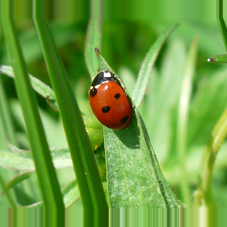
\includegraphics[width=2cm]{data/ladybug.png}
            };
            \draw[-Latex] (input) -- (model);

            \node[anchor=west] (output) at ($ (model.east) + (0.77, 0) $) {
                Ladybug
            };
            \draw[-Latex] (model) -- (output);
        }
        \only<3>{
            \neuron{n00}{red!25!black}{($ (model) + (-2 * \hsep, -2 * \vsep) $)}
            \neuron{n01}{red!90!black}{($ (model) + (-2 * \hsep, -\vsep) $)}
            \neuron{n02}{yellow!15!red}{($ (model) + (-2 * \hsep, 0) $)}
            \neuron{n03}{red!99!black}{($ (model) + (-2 * \hsep, \vsep) $)}
            \neuron{n04}{red!10!black}{($ (model) + (-2 * \hsep, 2 * \vsep) $)}

            \neuron{n10}{red!55!black}{($ (model) + (-\hsep, -1.5 * \vsep) $)}
            \neuron{n11}{yellow!20!red}{($ (model) + (-\hsep, -0.5 * \vsep) $)}
            \neuron{n12}{yellow!90!red}{($ (model) + (-\hsep, 0.5 * \vsep) $)}
            \neuron{n13}{red!7!black}{($ (model) + (-\hsep, 1.5 * \vsep) $)}

            \neuron{n20}{red!90!black}{($ (model) + (0, -\vsep) $)}
            \neuron{n21}{red!30!black}{(model)}
            \neuron{n22}{yellow!70!red}{($ (model) + (0, \vsep) $)}

            \neuron{n30}{yellow!40!red}{($ (model) + (\hsep, -0.5 * \vsep) $)}
            \neuron{n31}{red!65!black}{($ (model) + (\hsep, 0.5 * \vsep) $)}

            \neuron{n40}{red}{($ (model) + (2 * \hsep, 0) $)}

            \draw[stealth-, \edgecolor, opacity=\edgeopacity] (model.west) -- (n00);
            \draw[stealth-, \edgecolor, opacity=\edgeopacity] (model.west) -- (n01);
            \draw[stealth-, \edgecolor, opacity=\edgeopacity] (model.west) -- (n02);
            \draw[stealth-, \edgecolor, opacity=\edgeopacity] (model.west) -- (n03);
            \draw[stealth-, \edgecolor, opacity=\edgeopacity] (model.west) -- (n04);

            \foreach \i in {0,...,4} {
                \foreach \j in {0,...,3} {
                    \draw[\edgecolor, opacity=\edgeopacity] (n0\i) -- (n1\j);
                }
            }
            \foreach \i in {0,...,3} {
                \foreach \j in {0,...,2} {
                    \draw[\edgecolor, opacity=\edgeopacity] (n1\i) -- (n2\j);
                }
            }
            \foreach \i in {0,...,2} {
                \foreach \j in {0,...,1} {
                    \draw[\edgecolor, opacity=\edgeopacity] (n2\i) -- (n3\j);
                }
            }
            \foreach \i in {0,...,1} {
                \draw[\edgecolor, opacity=\edgeopacity] (n3\i) -- (n40);
            }

            \draw[stealth-, \edgecolor, opacity=\edgeopacity] (n40) -- (model.east);

            \node[anchor=east, draw=black, inner sep=0pt] (input) at ($ (model.west) + (-0.77, 0) $) {
                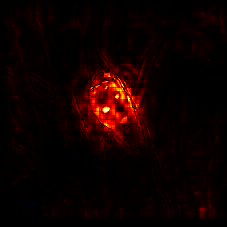
\includegraphics[width=2cm]{data/ladybug_explanation.png}
            };
            \draw[Latex-,red] (input) -- (model);

            \node[anchor=west, text=red] (output) at ($ (model.east) + (0.77, 0) $) {
                Ladybug
            };
            \draw[Latex-,red] (model) -- (output);
        }
    \end{tikzpicture}
\end{frame}

\begin{frame}{Dementia background}
    Dementia background
\end{frame}

\newcommand{\dementiadataset}{
    \begin{tikzpicture}
        \begin{axis}[
            width=\textwidth,
            height=0.4\textwidth,
            xmin=46,
            xmax=99,
            ymin=-1.6,
            ymax=1.2,
            xtick={55,60,65,70,75,80,85,90,95},
            axis lines=center,
            axis y line=none,
            clip=false
        ]
            \addplot[name path=zero, draw=none] coordinates {(47,0) (97,0)};

            \addplot[
                name path=fcases,
                draw=red,
                very thick
            ] table [
                col sep=comma,
                x=x,
                y=F-cases
            ]{data/dementia/dataset/dementia_full.csv};\label{trace:cases}
            \addplot[fill=red, opacity=0.2] fill between [of=zero and fcases];

            \addplot[
                name path=fcontrols,
                draw=blue,
                very thick
            ] table [
                col sep=comma,
                x=x,
                y=F-controls
            ]{data/dementia/dataset/dementia_full.csv};\label{trace:controls}
            \addplot[fill=blue, opacity=0.2] fill between [of=zero and fcontrols];

            \addplot[
                name path=mcases,
                draw=red,
                very thick
            ] table [
                col sep=comma,
                x=x,y
                expr=\thisrow{M-cases} * -1
            ]{data/dementia/dataset/dementia_full.csv};
            \addplot[fill=red, opacity=0.2] fill between [of=zero and mcases];

            \addplot[
                name path=mcontrols,
                draw=blue,
                very thick
            ] table [
                col sep=comma,
                x=x,
                y expr=\thisrow{M-controls} * -1
            ]{data/dementia/dataset/dementia_full.csv};
            \addplot[fill=blue, opacity=0.2] fill between [of=zero and mcontrols];

            \node[anchor=south west] at (axis cs: 46, 0.07) {\textbf{FEMALE}};
            \node[anchor=north west] at (axis cs: 46, -0.07) {\textbf{MALE}};
            \node[anchor=south, font=\footnotesize\selectfont, align=center] (n) at (axis cs: 72.5,-1.6) {n=1708};
            \node[anchor=south west,font=\footnotesize\selectfont, align=left] at ($(n.south east) + (110,0) $) {
                \ref{trace:controls} Controls\\[-0.1cm]
                \ref{trace:cases} Patients
            };
        \end{axis}
    \end{tikzpicture}
}

\newcommand{\scannersubplot}[3]{
    \nextgroupplot[
            axis lines=center,
            axis y line=none,
            xmin=46,
            xmax=99,
            ymin=-1.65,
            ymax=1.5,
            xmajorticks=false,
            axis line style={-}
        ]

            \addplot[name path=zero, draw=none] coordinates {(46, 0) (99, 0)};
            \addplot[
                name path=fcases,
                draw=red,
                very thick
            ] table [
                col sep=comma,
                x=x,
                y=F-cases
            ]{#1};
            \addplot[fill=red, opacity=0.2] fill between [of=zero and fcases];

            \addplot[
                name path=fcontrols,
                draw=blue,
                very thick
            ] table [
                col sep=comma,
                x=x,
                y=F-controls
            ]{#1};
            \addplot[fill=blue, opacity=0.2] fill between [of=zero and fcontrols];

            \addplot[
                name path=mcases,
                draw=red,
                very thick
            ] table [
                col sep=comma,
                x=x,
                y expr=\thisrow{M-cases} * -1
            ]{#1};
            \addplot[fill=red, opacity=0.2] fill between [of=zero and mcases];

            \addplot[
                name path=mcontrols,
                draw=blue,
                very thick
            ] table [
                col sep=comma,
                x=x,
                y expr=\thisrow{M-controls} * -1
            ]{#1};
            \addplot[fill=blue, opacity=0.2] fill between [of=zero and mcontrols];

            \node[anchor=south] at (axis cs: 72.5,1) {\tiny{#2}};
            \node[anchor=north] at (axis cs: 72.5,-1) {\tiny{\textbf{n=#3}}};
}

\newcommand{\dementiasubsets}{
    \begin{tikzpicture}
        \begin{groupplot}[
            group style={
                group size=5 by 2,
                horizontal sep=0.25cm,
                vertical sep=0.25cm
            },
            height=0.314\textwidth,
            width=0.314\textwidth
        ]
            \scannersubplot{data/dementia/dataset/dementia_ADNI_30T.csv}{ADNI 3.0T}{506}
            \scannersubplot{data/dementia/dataset/dementia_oasis3_30T.csv}{OASIS3 3.0T}{438}
            \scannersubplot{data/dementia/dataset/dementia_ADNI_15T.csv}{ADNI 1.5T}{290}
            \scannersubplot{data/dementia/dataset/dementia_Oslo_GE750.csv}{Oslo GE750}{226}
            \scannersubplot{data/dementia/dataset/dementia_AIBL_10.csv}{AIBL Site 1}{92}
            \scannersubplot{data/dementia/dataset/dementia_addneuromed_GE_MEDICAL_SYSTEMS.csv}{ANM GE}{74}
            \scannersubplot{data/dementia/dataset/dementia_miriad_15_T_Signa.csv}{MIRIAD}{38}
            \scannersubplot{data/dementia/dataset/dementia_AIBL_20.csv}{AIBL Site 2}{22}
            \scannersubplot{data/dementia/dataset/dementia_addneuromed_PICKER_International_Inc.csv}{ANM Picker}{12}
            \scannersubplot{data/dementia/dataset/dementia_oasis3_15T.csv}{OASIS3 1.5T}{10}
        \end{groupplot}
    \end{tikzpicture}
}


\newcommand{\diceplot}[1]{
    \def\legendsize{\footnotesize}
    \def\legendnodesep{2pt}
    \def\legenddistance{1}

    \begin{tikzpicture}
        \begin{axis}[
            width=7cm,
            height=7cm,
            ylabel=\footnotesize{Dice coefficient},
            xlabel=\footnotesize{Binarization threshold percentile},
            ymin=0,
            ymax=1,
            xmin=0,
            xmax=0.99,
            tick label style={font=\scriptsize},
            xtick={0, 0.2, 0.4, 0.6, 0.8, 0.99},
            xticklabels={0, 20, 40, 60, 80, 99},
            xtick style={draw=none},
            ytick style={draw=none},
            xmajorgrids=true,
            ymajorgrids=true
        ]
            \addplot[very thick,draw=dementiadice] table [col sep=comma, x=thresholds, y=test] {data/dice.csv};\label{trace:dementia}

            \ifnum#1=1
                \addplot[very thick,draw=sexdice] table [col sep=comma, x=thresholds, y=sex] {data/dice.csv};\label{trace:sex}
                \addplot[very thick,draw=weightsdice] table [col sep=comma, x=thresholds, y=randomized_weights] {data/dice.csv};\label{trace:weights}
                \addplot[very thick,draw=imagesdice] table [col sep=comma, x=thresholds, y=randomized_images] {data/dice.csv};\label{trace:images}
            \fi

            \addplot[only marks, fill=dementiadice, draw=dementiadice, mark size=3] coordinates {
                (0.5, 0.6131)
                (0.7, 0.5296)
                (0.9, 0.4291)
            };
            \node[anchor=north, inner sep=01, fill=white, draw=black] at (axis cs: 0.5,0.5831) {\legendsize{0.61}};
            \node[anchor=north, inner sep=\annotationpadding] at (axis cs: 0.7,0.5296) {\legendsize{0.52}};
            \node[anchor=north, inner sep=\annotationpadding] at (axis cs: 0.9,0.4191) {\legendsize{0.41}};
            \node[anchor=south, inner sep=\annotationpadding] at (axis cs: 0.5,0.6131) {
                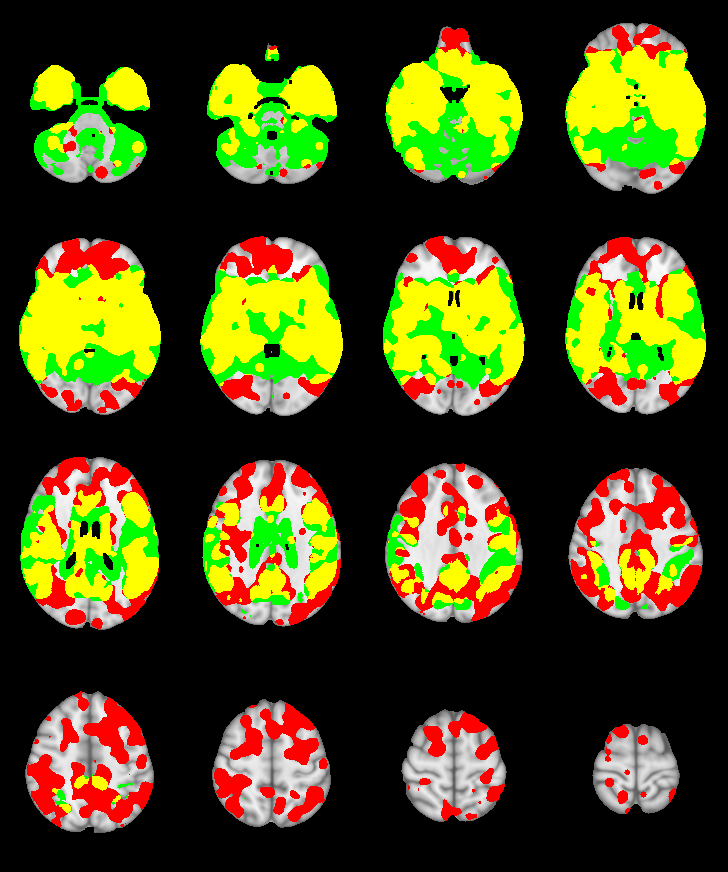
\includegraphics[
                    width=\slicewidth,
                    clip=true,
                    trim = 192mm 232mm 0mm 0mm
                ]{data/test_50.png}
            };
            \node[anchor=south, inner sep=\annotationpadding] at (axis cs: 0.7,0.5296) {
                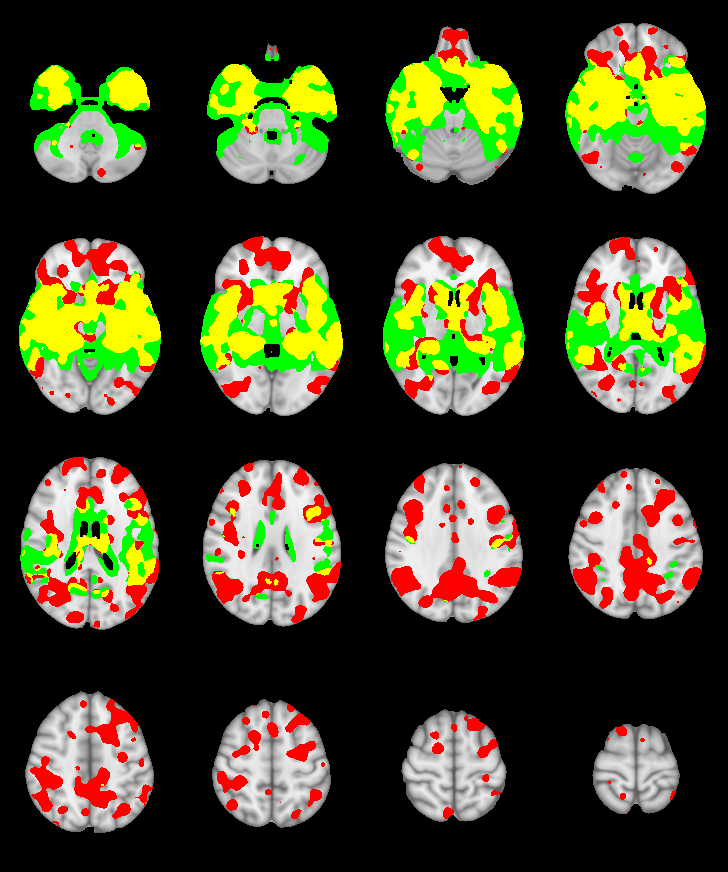
\includegraphics[
                    width=\slicewidth,
                    clip=true,
                    trim = 192mm 232mm 0mm 0mm
                ]{data/test_70.png}
            };
            \node[anchor=south, inner sep=\annotationpadding] at (axis cs: 0.9,0.4291) {
                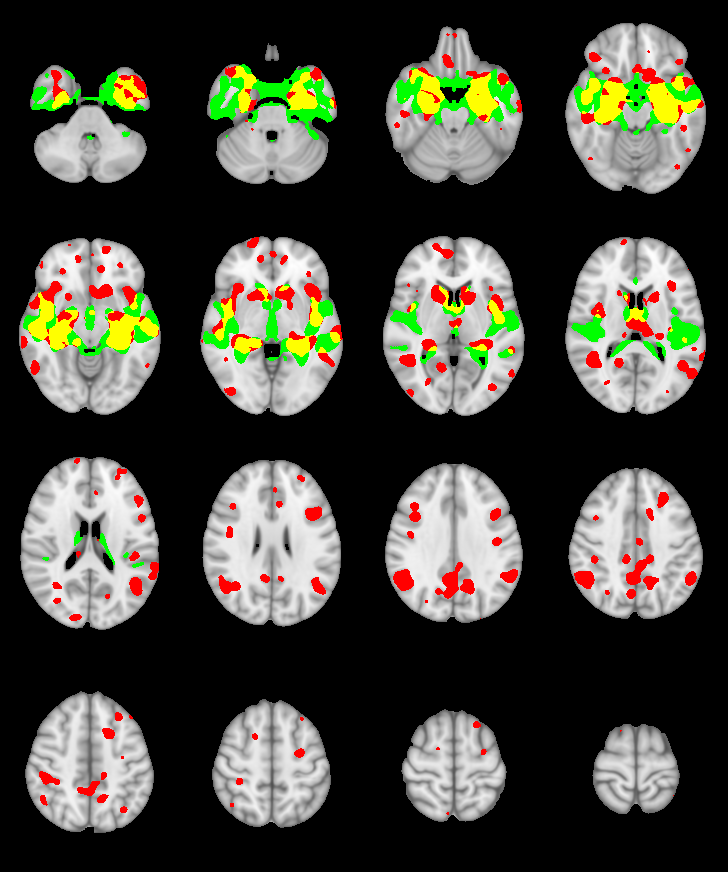
\includegraphics[
                    width=\slicewidth,
                    clip=true,
                    trim = 192mm 232mm 0mm 0mm
                ]{data/test_90.png}
            };
            % Legend
            \ifnum#1=1
                \node[
                    anchor=south west,
                    draw=black,
                    fill=white,
                    minimum width=3.45cm,
                    minimum height=1.22cm
                ] at (axis cs: 0.015, 0.015) {};
                \node[
                    circle,
                    draw=imagesdice,
                    fill=imagesdice,
                    anchor=south west,
                    inner sep=\legendnodesep
                ] (rwnode) at (axis cs: 0.035, 0.045) {};
                \node[anchor=west, text depth=0] (rw) at (rwnode.east) {\legendsize{Randomized images}};
                \node[
                    circle,
                    draw=weightsdice,
                    fill=weightsdice,
                    anchor=south,
                    inner sep=\legendnodesep
                ] (rinode) at ($ (rwnode.north) + (0, \legenddistance) $) {};
                \node[anchor=west, text depth=0] at (rinode.east) {\legendsize{Randomized weights}};
                \node[
                    circle,
                    draw=sexdice,
                    fill=sexdice,
                    anchor=south,
                    inner sep=\legendnodesep
                ] (sexnode) at ($ (rinode.north) + (0, \legenddistance) $) {};
                \node[anchor=west, text depth=0] at (sexnode.east) {\legendsize{Sex}};
                \node[
                    circle,
                    draw=dementiadice,
                    fill=dementiadice,
                    anchor=south,
                    inner sep=\legendnodesep
                ] (demnode) at ($ (sexnode.north) + (0, \legenddistance) $) {};
                \node[anchor=west, text depth=0] at (demnode.east) {\legendsize{Dementia}};
            \fi
        \end{axis}
    \end{tikzpicture}
}

\newcommand{\dementiapredictions}{
    \newcommand{\ymin}{-0.35}
    \newcommand{\ymax}{1.05}

    \begin{tikzpicture}
        \begin{axis}[
            name=distributions,
            height=0.5\textwidth,
            width=0.94\textwidth,
            xtick pos=bottom,
            ymajorticks=false,
            xmin=0,
            xmax=1,
            ymin=\ymin,
            ymax=\ymax,
            xlabel=\small{Predicted probability of dementia},
            every tick label/.append style={font=\small}
        ]
            \addplot[
                name path=controls,
                draw=blue,
                very thick
            ] table [
                col sep=comma,
                x=prediction,
                y=controls
            ]{data/dementia/test_distributions.csv};

            \addplot[
                name path=cases,
                draw=red,
                very thick
            ] table [
                col sep=comma,
                x=prediction,
                y=cases
            ]{data/dementia/test_distributions.csv};

            \addplot[name path=zero, draw=black] coordinates {(0,0) (1,0)};
            \addplot[fill=blue, opacity=0.2] fill between [of=zero and controls];
            \addplot[fill=red, opacity=0.2] fill between [of=zero and cases];

            \addplot[
                scatter/classes={
                    control={blue, draw=black, opacity=0.5},
                    case={red, draw=black, opacity=0.5}
                },
                scatter,
                mark=*,
                only marks,
                point meta=explicit symbolic
            ] table [
                col sep=comma,
                y expr=\thisrow{y} * -0.15 - 0.1,
                meta=class,
            ] {data/dementia/test_predictions.csv};
            \addplot[dashed] coordinates {(0.5, \ymin) (0.5, \ymax)};
        \end{axis}

        \node[anchor=south west] at ($ (distributions.south east) + (0,0.45) $) {\footnotesize{Controls}};
        \node[anchor=south west] at ($ (distributions.south east) + (0,0.0) $) {\footnotesize{Cases}};
    \end{tikzpicture}
}


\begin{frame}{Modelling}
    \begin{tikzpicture}
        \node[] at (-5.25, -3.5) {};
        \node[] at (5.25, 3.5) {};

        \only<1>{
            \node[anchor=north] at (0, 3.5) {
                \dementiadataset
            };
            \node[] at (0, -1.5) {
                \dementiasubsets
            };
        }
        \only<2,4>{
            \node[] at (0, 0) {
                \cnnbox{0}{Patient or healthy control}
            };
        }
        \only<3>{
            \node[] at (0, 0) {
                \dementiapredictions
            };
        }
        \only<5>{
            \node[] at (0, 0) {
                \cnnbox{1}{Patient or healthy control}
            };
        }
        \only<6>{
			\node[
				minimum height=0.41\textwidth,
				minimum width=0.32\textwidth,
				fill=black,
                anchor=west
			] (box1) at (-5.25, 0) {};
			\node[anchor=south] at (box1.south) {
				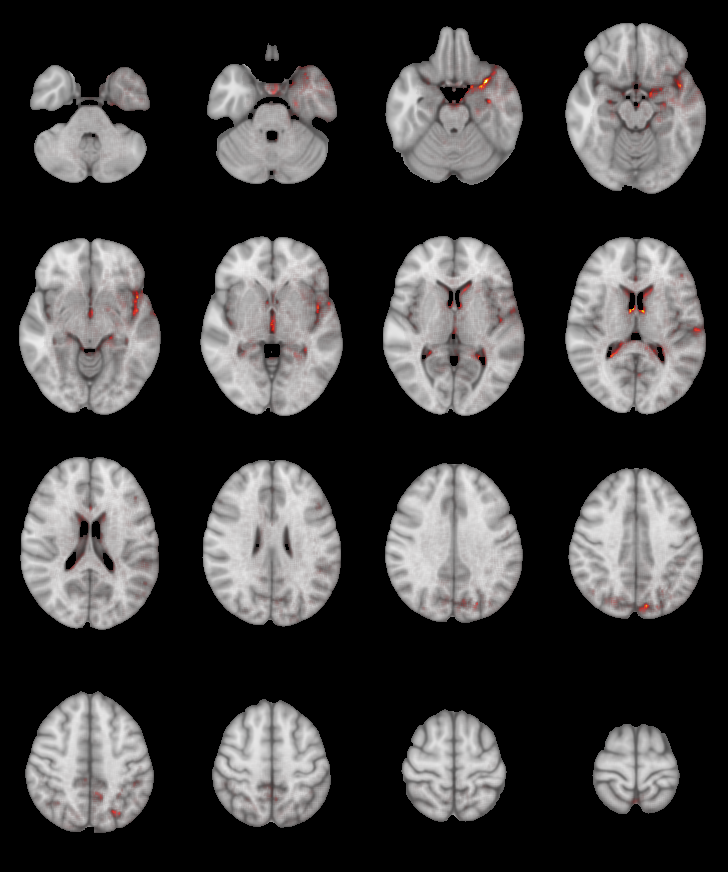
\includegraphics[width=0.31\textwidth]{data/dementia/subject1.png}
			};
			\node[anchor=north,inner sep=2pt, text=white, font=\footnotesize] at (box1.north) {Patient 1};

			\node
				[minimum height=0.41\textwidth,
				minimum width=0.32\textwidth,
				fill=black,
				anchor=west
			] (box2) at ($ (box1.east) + (0.05,0) $) {};
			\node[anchor=south] at (box2.south) {
				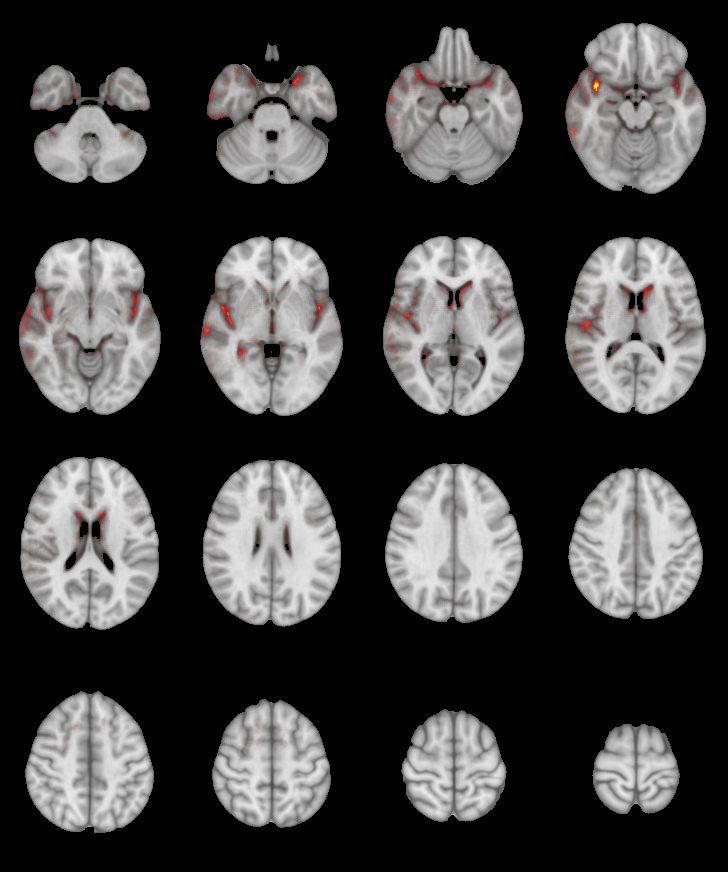
\includegraphics[width=0.31\textwidth]{data/dementia/subject2.png}
			};
			\node[anchor=north,inner sep=3pt, text=white, font=\footnotesize] at (box2.north) {Partient 2};

			\node
				[minimum height=0.41\textwidth,
				minimum width=0.32\textwidth,
				fill=black,
				anchor=west
			] (box3) at ($ (box2.east) + (0.05,0) $) {};
			\node[anchor=south] at (box3.south) {
				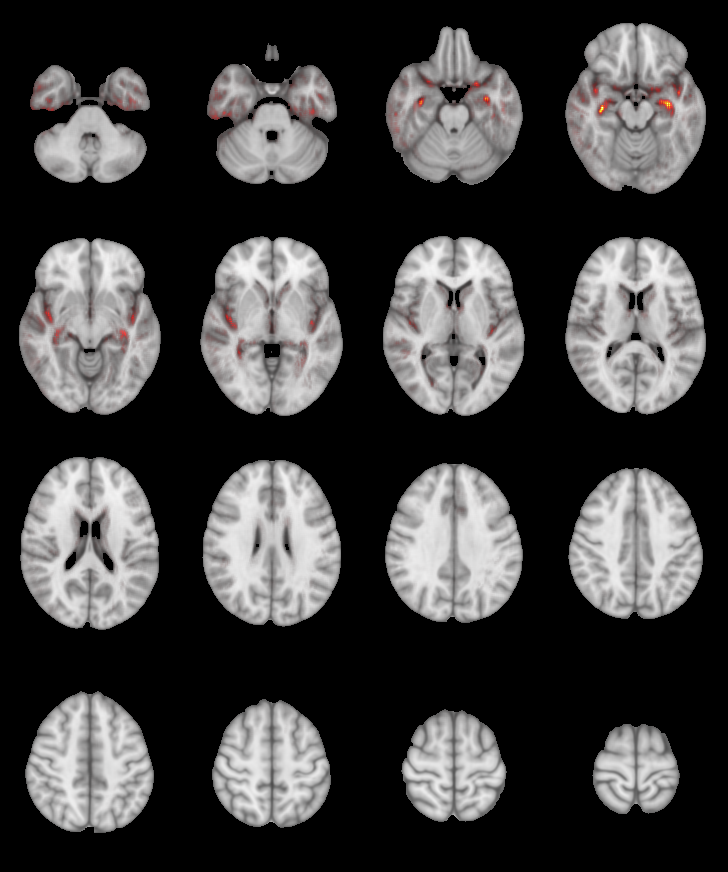
\includegraphics[width=0.31\textwidth]{data/dementia/subject3.png}
			};
			\node[anchor=north,inner sep=3pt, text=white, font=\footnotesize] at (box3.north) {Patient 3};
        }
         \visible<7-8>{
            \node[label={[text depth=0]above:LRP}] at (-2.25, 0) {
				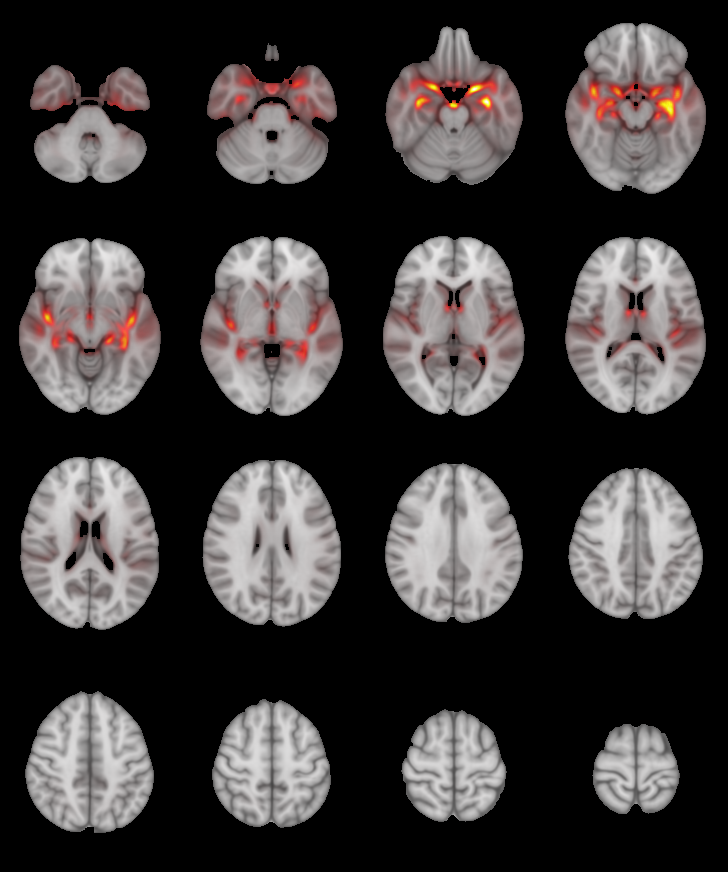
\includegraphics[width=0.31\textwidth]{data/dementia/dementia_average.png}
			};
        }
        \visible<8>{
			\node[label={[text depth=0]above:GingerALE}] at (2.25, 0) {
				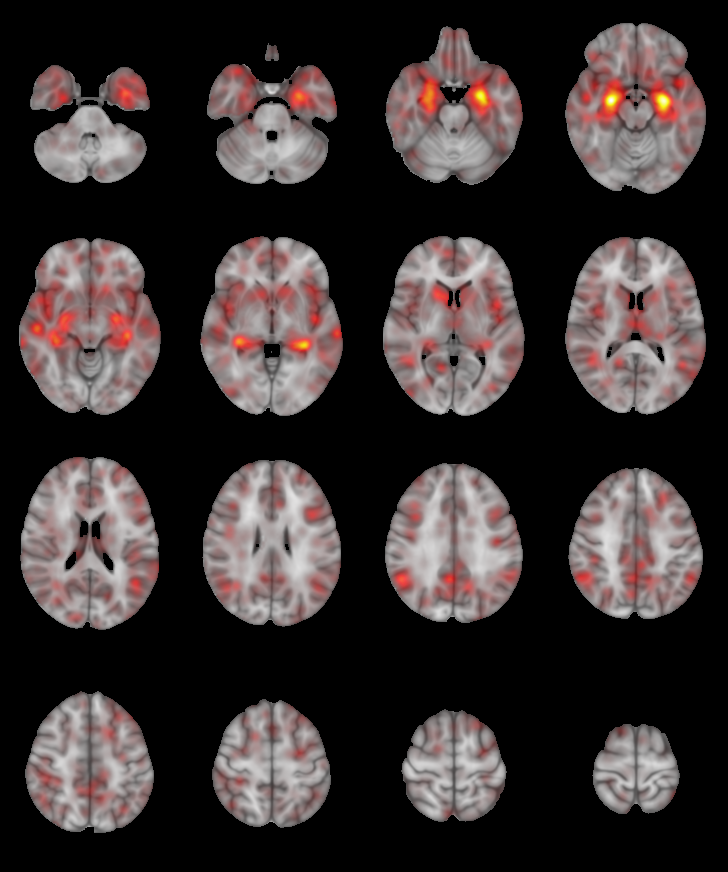
\includegraphics[width=0.31\textwidth]{data/dementia/ALE.png}
			};
        }
    \end{tikzpicture}
\end{frame}
